\section{Основные понятия, простейшие типы дифференциальных уравнений.}

\subsection{Основные понятия. Простейшие типы уравнений первого порядка: уравнения с разделяющимися переменными, однородные, линейные.}
Рассмотрим функцию $y(x)$, определённую вместе с $n$ производными на промежутке $I$. \newline Также рассмотрим функцию $F(x,y,p_1, \ldots,p_n)$, определённую и непрерывную на некотором $\Omega\subset \R^{n+2}$

\Def Уравнение вида 
\setcounter{equation}{0}
\begin{equation}\label{eq1} 
    F(x, y, y', \ldots, y^{(n)})=0
\end{equation}
называется \textit{дифференциальным уравнением $n$-го порядка}.

\Def Функция $\varphi(x)$, определённая на $I$ вместе со своими $n$ производными,
называется решением уравнения (\ref{eq1}), если:
\begin{enumerate}
    \item $\varphi$ и все её $n$ производных непрерывны на $I$.
    \item $\forall x \in I \quad (x, \varphi(x), \varphi'(x), \ldots, \varphi^{n}(x)) \in \Omega$
    \item $\forall x \in I \quad F(x, \varphi(x), \varphi'(x), \ldots, \varphi^{n}(x)) = 0$
\end{enumerate}

\Def \textit{Обыкновенным дифференциальным уравнением I-го порядка} называется уравнение вида $F(x,y,y') = 0$

\Def $y'=\frac{dy}{dx}=f(x,y)$ -- \textit{уравнение, разрешённое относительно производной}

\Def Функция $y = \varphi(x)$, определенная на промежутке $I$, называется \textit{решением дифференциального уравнения} $y'=f(x,y)$, если 
\begin{enumerate}
    \item $\varphi$ имеет непрерывную производную $\varphi'(x)$ на $I$.
    \item $\forall x \in I \quad (x, \varphi(x)) \in \Omega$
    \item $\varphi'(x) = f(x,\varphi(x))$ на $I$
\end{enumerate}

\Def $M(x,y)dx + N(x,y)dy = 0$ -- \textit{уравнение в дифференциалах}. Подмножество его решений:
\begin{equation*}
    \left[ 
      \begin{gathered} 
        y_x' = -\frac{M(x,y)}{N(x,y)} \\ 
        x_y' = -\frac{N(x,y)}{M(x,y)} \\ 
      \end{gathered} 
\right.
\end{equation*}





\subsection*{Уравнения с разделяющимися переменными}

Уравнения с разделяющимися переменными -- это уравнения, которые могут быть записаны в виде
\begin{equation}\label{eq2} 
    y' = f(x)g(y) \qquad f(x) \in C(I_1), g(y) \in C(I_2)
\end{equation}
\begin{center}
    или же в виде
\end{center}
\begin{equation}\label{eq3} 
    M(x)N(y)dx + P(x)Q(y)dy = 0
\end{equation}

\Note Если же $y_k\in I_2$ решение уравнение $g(y) = 0$, то $y\equiv y_k$ -- решение дифф. уравнения.
\bigbreak
Если же $y(x)$ нигде не принимает значение $y_k$, то $g(y) \neq 0$, а потому мы можем делить на него. Значит, чтобы решить исходное уравнение, необходимо \textit{разделить переменные}, то есть, привести уравнение к такой форме, чтобы при дифференциале $dx$ стояла
функция, зависящая лишь от $x$, а при дифференциале $dy$ -- функция, зависящая от $y$. 

Для этого уравнение вида (\ref{eq2}) или (\ref{eq3}) следует переписать в форме:

\begin{equation*}
    \frac{y'}{g(y)} = f(x) \qquad \qquad \frac{M(x)}{P(x)}dx + \frac{Q(y)}{N(y)}dy = 0
\end{equation*}

Будем работать с первым вариантом, так как он более общий. Проинтегрируем обе части по $x$:
\begin{align*}
    \int\frac{y'dx}{g(y)} &= \int f(x)dx \\
    \int\frac{dy}{g(y)} &= \int f(x)dx \\
    H(y) &= F(x) + C \\
    y &= H^{-1}(F(x) + C)
\end{align*}

Поскольку $g(y)$ знакопостоянна, то $H(y)$ строго монотонна, а следовательно, обратима

\subsection*{Уравнения, приводящиеся к уравнениям с разделяющимися переменными}
\begin{equation*}
    y' = f(ax + by + c)
\end{equation*}
Сделав в таком уравнении замену $z = ax + by + c$, получим уравнение с разделяющимися переменными $\frac{dz}{dx} = bf(z) + a$.


\subsection*{Однородные уравнения}
\Def Функция двух переменных $f(x, y)$ называется \textit{однородной степени} $m$ (еще
говорят, с показателем однородности $m$), если для всех $t$ (или хотя бы для
$t > 0$) справедливо соотношение: 
\begin{center}
    $f(tx, ty) = t^m f(x, y)$
\end{center} 

\textit{Однородным дифференциальным уравнением} называется уравнение вида 
\begin{equation}
    M(x, y) dx + N(x, y) dy = 0
\end{equation}
если $M(x, y)$ и $N(x, y)$ -- однородные функции одной и той же степени $m$. 

Можно показать, что однородное уравнение может
также быть записано в виде 
\begin{center}
    $y' = f(\frac{y}{x}), \qquad f(z)\in C(I)$
\end{center}

Однородное уравнение приводится к уравнению с разделяющимися переменными с помощью замены искомой функции $y(x)$ по формуле:
\begin{center}
    $t(x) = \frac{y(x)}{x}$
\end{center}

Тогда производная $y'$ и дифференциал $dy$ заменяются по формулам:
\begin{equation*}
    y' = t'x + t, \qquad dy = tdx + xdt
\end{equation*}
После решения полученного уравнения нужно сделать обратную подстановку $t = \frac{y}{x}$


\subsection*{Уравнения, приводящиеся к однородным}
\begin{equation*}
    y' = f\Big(\frac{ax + by + c}{a_1x + b_1y + c_1}\Big), \qquad f(z)\in C(I)
\end{equation*}
приводится к однородному уравнению заменой $u = x - x_0, \; v = y - y_0$ , где $(x_0, y_0)$ — точка пересечения прямых $ax+by+c = 0$ и $a_1x+b_1y+c_1 = 0$. Если
же эти прямые не пересекаются, то $a_1x + b_1y = k(ax + by)$ для некоторого $k \in \R$ и уравнение имеет вид $y' = f_1(ax+by)$.

\Def Уравнение называется \textit{обобщенно-однородным}, если его можно привести к
однородному заменой $y = z^m$ , где $m$ -- некоторое действительное число.

\Example $9yy' - 18xy + 4x^3 = 0 \;\; \Rightarrow \;\; 9mz^{2m-1}z'-18xz^m+4x^3 = 0$. 

Оно однородно, если $2m-1 = 1+m = 3 \;\; \Rightarrow \;\; m = 2 \;\; \Rightarrow \;\; 9z^3z' - 9xz^2 + 2x^3 = 0.$




\subsection*{Линейные уравнения}

\textit{Линейным уравнением первого порядка} называется уравнение, линейное относительно искомой функции $y(x)$ и ее производной, то есть, уравнение вида
\begin{equation}\label{eq5}
    y' + a(x)y = b(x) \qquad a(x), b(x) \in C(I)
\end{equation}

Функция $b(x)$ называется \textit{свободным членом} уравнения (4). Уравнение 
\begin{equation}\label{eq6}
    y' + a(x)y = 0
\end{equation}
называется \textit{линейным однородным уравнением}, соответствующим линейному уравнению (\ref{eq5}).

Покажем, что однородное уравнение является уравнением с разделяющимися переменными (далее подразумевается, что $y \neq 0$):
\begin{align*}
    y' + a(x)y &= 0 \qquad \Rightarrow \qquad
    \frac{y'}{y} = -a(x) \qquad \Rightarrow \qquad
    \int\frac{dy}{y} = -\int a(x)dx \qquad \Rightarrow\\
    \Rightarrow \qquad \ln|y| &= -\int\limits_{x_0}^xa(t)dt + C \qquad \Rightarrow \qquad
    |y| = e^{C}\cdot e^{-\int\limits_{x_0}^xa(t)dt}
\end{align*}
Работаем с интегралом с переменным верхним пределом ($x_0$ -- любая точка из промежутка непрерывности $a(t)$). Таким образом, мы получили одну из возможных первообразных, а все остальные с помощью прибавления константы.

Объединяя все решения, получаем \textit{общее решение}:
\begin{equation*}
    y_0=C\exp{\Big[-\int\limits_{x_0}^xa(t)dt\Big]}
\end{equation*}
Будем искать частное решение исходного линейного уравнения в виде 

\textbf{метод вариации постоянной}:
\begin{equation*}
    y_{\text{ч}}=C(x)\cdot\exp{\Big[-\int\limits_{x_0}^xa(t)dt\Big]}
\end{equation*}

Подставим его в левую часть уравнения:
\begin{align*}
    y' + a(x)y = \exp{\Big[-\int\limits_{x_0}^xa(t)dt\Big]}\cdot \Big(C'(x) - C(x)a(x) + C(x)a(x)\Big) 
    = C'(x)\cdot \exp{\Big[-\int\limits_{x_0}^xa(t)dt\Big]}
\end{align*}
Тогда получаем, что исходное уравнение (\ref{eq5}) имеет вид:
\begin{align*}
    C'(x) &= b(x) \cdot \exp{\Big[\int\limits_{x_0}^xa(t)dt\Big]}\\
    C(x) &= \int\limits_{x_1}^{x}b(t)\exp{\Big[\int\limits_{t_0}^ta(\tau)d\tau\Big]}dt + C \\
    y &= \underbrace{\Big(\int\limits_{x_1}^{x}b(t)\exp{\Big[\int\limits_{t_0}^ta(\tau)d\tau\Big]}dt\Big)\cdot \exp{\Big[-\int\limits_{x_0}^xa(t)dt\Big]}}_{\text{частного решение линейного}} + \underbrace{C\exp{\Big[-\int\limits_{x_0}^xa(t)dt\Big]}}_{\text{общее решение однородного}}
\end{align*}

\Example $y' + y = 4x$

Решение однородного: $y = Ce^{-x}$

Подстановка: $C'(x)e^{-x} - C(x)e^{-x} + C(x)e^{-x} = 4x \;\; \Rightarrow \; C'(x) = 4xe^{x}$
\begin{align*}
    C(x) &= 4(xe^x - \smallint e^xdx) = 4(x-1)e^x + C \\
    y &= 4(x-1) + Ce^{-x}
\end{align*}

\newpage

\subsection{Уравнения в полных дифференциалах. Интегрирующий множитель. Уравнения Бернулли и Риккати}
\subsection*{Уравнения в полных дифференциалах}
Рассмотрим уравнение первого порядка, записанное в дифференциалах. Это уравнение
\begin{equation}\label{eq7}
    M(x, y) dx + N(x, y) dy = 0
\end{equation}
называется \textit{уравнением в полных дифференциалах}, если его левая часть является дифференциалом некоторой гладкой функции $F(x, y)$. 
Тогда это уравнение
можно переписать в виде $dF(x, y) = 0$, так что его решение будет иметь вид
\begin{equation*}
    F(x, y) = C
\end{equation*}

\Statement Если функции $M(x, y)$ и $N(x, y)$ определены и непрерывны в некоторой односвязной области $\Omega$ и имеют в ней \underline{непрерывные частные производные} по $x$ и по $y$, то уравнение (\ref{eq7}) будет уравнением в полных дифференциалах тогда и только тогда, когда выполняется тождество
\begin{equation}\label{eq8}
    \frac{\partial M(x,y)}{\partial y} \equiv \frac{\partial N(x,y)}{\partial x}
\end{equation}

Легко понять откуда берется это тождество: если $F$ — решение уравнения, то 
\[
M(x, y) = \frac{\partial F}{\partial x}, \;\; N(x, y) = \frac{\partial F}{\partial y}.
\]
Тогда 
\[
\frac{\partial M(x,y)}{\partial y} =  \frac{\partial^2 F}{\partial x \partial y} = \frac{\partial N(x,y)}{\partial x}.
\]

Если это условие выполнено, то криволинейный интеграл
\begin{equation*}
    \int\limits_{(x_0, y_0)}^{(x,y)}M dx + N dy
\end{equation*}
не зависит от выбора пути интегрирования, поэтому функцию $F(x, y)$ можно восстановить по любой из формул
\begin{equation}\label{eq9}
    F(x, y) = \int\limits_{x_0}^xM(x, y) dx + \int\limits_{y_0}^yN(x_0, y) dy \qquad \text{или} \qquad F(x, y) = \int\limits_{y_0}^yN(x, y) dx + \int\limits_{x_0}^xM(x, y_0) dy
\end{equation}

При этом нижние пределы $x_0$ и $y_0$ можно выбирать произвольно, лишь бы точка $(x_0, y_0)$ принадлежала области $D$ (области определения функций $M$
и $N$). За счет правильного выбора чисел $x_0$ и $y_0$ иногда удается упростить
вычисления интегралов (\ref{eq9}). Например, если функции $M$ и $N$ являются многочленами от $x$ и $y$, целесообразно выбирать $x_0 = y_0 = 0$.

\subsection*{Интегрирующий множитель}
Пусть дано уравнение~(\ref{eq7}), для которого не выполнено условие (\ref{eq8}).

\Def Функция $\mu(x, y) \neq 0$ называется \textit{интегрирующим множителем} для уравнения (\ref{eq7}), если уравнение
\begin{equation*}
    \mu(x, y)\big(M(x, y) dx + N(x, y) dy\big) = 0,
\end{equation*}
является уравнением в полных дифференциалах. Отсюда следует, что функция $\mu$ удовлетворяет условию
\begin{equation*}
    \frac{\partial(\mu M)}{\partial y} \equiv \frac{\partial(\mu N)}{\partial x}
\end{equation*}

Это равенство дает уравнение в частных производных первого порядка для $\mu(x,y)$:
\begin{equation*}
    N\frac{\partial\mu}{\partial x} - M\frac{\partial\mu}{\partial y} = \Big(\frac{\partial M}{\partial y} - \frac{\partial N}{\partial x}\Big)\mu
\end{equation*}
Поделив обе части последнего уравнения на $\mu$, перепишем его в виде:
\begin{equation*}
    N\frac{\partial(ln\mu)}{\partial x} - M\frac{\partial(ln\mu)}{\partial y} = \frac{\partial M}{\partial y} - \frac{\partial N}{\partial x}
\end{equation*}

Несмотря на то, что эти уравнения, как
правило, имеют бесконечно много решений, задача их нахождения в общем случае ничуть не легче решения исходного уравнения.

Рассмотрим два случая, когда уравнение (\ref{eq7}) имеет интегрирующий множитель, зависящий только от $x$ или только от $y$:
\begin{enumerate}
    \item $\mu = \mu(x)$. Тогда 
    \begin{equation*}
        \frac{d(ln\mu)}{d x} = \frac{\frac{\partial M}{\partial y} - \frac{\partial N}{\partial x}}{N}
    \end{equation*}
    и такой множитель существует, если правая часть зависит только от $x$ или
является постоянной.
    \item $\mu = \mu(y)$. Тогда 
    \begin{equation*}
        \frac{d(ln\mu)}{d y} = \frac{\frac{\partial M}{\partial y} - \frac{\partial N}{\partial x}}{-M}
    \end{equation*}
    и правая часть должна зависеть только от $y$ или быть постоянной.
\end{enumerate}

\subsection*{Уравнение Бернулли}
Нелинейное уравнение первого порядка вида
\begin{equation*}
    y' + a(x)y = b(x)y^m, \qquad m \neq 0, m \neq 1,\;\; a,b\in C(I)
\end{equation*}
называется \textit{уравнением Бернулли}. 
\bigbreak
Заметим, что $y=0$ -- решение
уравнения Бернулли при $m > 0$. 

Если $y \neq 0$, то, разделив уравнение на
$y^m$ и вводя новую неизвестную функцию $z = y^{1-m}$, относительно функции $z$ получаем линейное уравнение:
\begin{align*}
    \frac{y'}{y^m}+a(x)\frac{1}{y^{m-1}}=b(x)\qquad \text{при этом \;} (y^{1-m})'=(1-m)y^{-m}y' \\ 
    \text{Делаем замену: $z = y^{1-m}$} \quad \Rightarrow \qquad \frac{z'}{1-m}+a(x)z=b(x)
\end{align*}

\subsection*{Уравнение Риккати}
Нелинейное уравнение первого порядка вида
\begin{equation*}
    y' = a(x)y^2 + b(x)y + c(x), \qquad a,b,c\in C(I)
\end{equation*}
называется \textit{уравнением Риккати}. 
\bigbreak
В отличие от всех уравнений, рассматривавшихся ранее, уравнение Риккати не всегда интегрируется в квадратурах.
Чтобы решить его, необходимо знать хотя бы одно частное решение $y = y_1(x)$
этого уравнения. Тогда замена $y = y_1 + z$ приводит это уравнение к уравнению Бернулли. Однако, проще сразу сделать замену:
\begin{equation*}
    z = \frac{1}{y-y_1} \quad \Rightarrow \quad y = y_1+\frac{1}{z} \quad y'_x = y'_{1x} - \frac{z'_x}{z^2}
\end{equation*}
которая сводит уравнение Риккати к линейному.
\newpage

\subsection{Метод введения параметра для уравнения первого порядка, не разрешенного относительно производной}
\textbf{Определение} Уравнение первого порядка, не разрешенное относильно производной~--- это уравнение вида 
\begin{equation}\label{firstorder-parapm-eq}
    F(x, y, y') = 0
\end{equation}
где \(F(x, y, p)\)~--- заданная непрерывная функция в некоторой непустой окрестности $G$ евклидового пространства $\mathbb{R}_{(x, y, p)}^3$ с декартовыми прямоугольными координатами $x, y, p$. Где $x$~--- аргумент, $y = y(x)$~--- неизвестная функция.

В общем случае для решения уравнения~(\ref{firstorder-parapm-eq}) применяется метод введения параметра, который позволяет свести решение~(\ref{firstorder-parapm-eq}) к решению некоторого уравнения первого порядка в симметричной форме.

Сам метод: положим $y' = p$ и рассмотрим систему
\begin{equation}\label{firstorder-parapm-sys}
    \begin{cases}
    F(x, y, p) = 0 \\
    dy = pdx.
    \end{cases}
\end{equation}

\begin{theorem}[Не доказывалось]
Уравнение~(\ref{firstorder-parapm-eq}) эквивалентно системе~(\ref{firstorder-parapm-sys}).
\end{theorem}
\begin{proof}
Проверяется непосредственной подстановкой решений.
\end{proof}

Наиболее важным является случай когда уравнение~(\ref{firstorder-parapm-eq}) разрешимо относительно $y$ или $x$. Тогда система~(\ref{firstorder-parapm-sys}) принимает вид 

\begin{equation}\label{firstorder-parapm-sys-simp}
    \begin{cases}
    y = f(x, p) \\
    dy = pdx.
    \end{cases}
\end{equation}
откуда получается уравнение
\[\left(\frac{\partial f}{\partial x} - p\right) dx + \frac{\partial f}{\partial p} dp = 0.\]

\begin{lemmanote}
При таком типе решения ошибкой является переход от параметра $p$ обратно к $y'$. Важно понимать, что это не замена, а именно введение параметра и решения могут быть записаны как в параметрической так и в явной форме.
\end{lemmanote}

\begin{lemmanote}[О возникновении неоднозначности]
Откуда берутся особые решения? При переходе к параметру $p$ неявно применяется теорема о неявной функции:
\begin{align*}
    F(x, y, p) &= 0 \; \Longleftrightarrow \; \underbrace{y' = p = f(x, y)}_{\text{т. о неявной функ.}}\\
    F(x, y, f(x, y)) &= 0.
\end{align*}
Но понятно, что у теоремы есть условия которые не всегда выполняются. В качестве примера можно рассмотерть уравнение $(y')^2 - x^2 = 0$.
\end{lemmanote}

\begin{theorem}
Пусть в области $G \subset \mathbb{R}^3$ функция $F$ непрерывна вместе с $\frac{\partial F}{\partial y}$, $\frac{\partial F}{\partial p}$, а также $\frac{\partial F}{\partial p}|_{(x_0, y_0, p_0) \in G} \neq 0$.
Тогда существует $\delta > 0$ на $[x_0 - \delta, x_0 + \delta]$ существует единственное решение задачи Коши
\[
\begin{cases}
F(x, y, y') = 0\\
F(x_0, y_0, p_0) = 0\\
y(x_0) = y_0\\
y'(x_0) = p_0
\end{cases}
\]
\end{theorem}
\begin{proof}
Так как $\frac{\partial F}{\partial p}|_{(x_0, y_0, p_0) \in G} \neq 0$, то по теореме о неявной функции $\exists U(x_0, y_0), U(p_0)$, что $p_0 = f(x_0, y_0)$ и 
\[\forall (x, y) \in U(x_0, y_0)\;\; \exists f(x, y): U(x_0, y_0) \rightarrow U(p_0), \; p = f(x, y).\]

Итого имеем
\[
\begin{cases}
y' = f(x, y)\\
y(x_0) = y_0.
\end{cases}
\]

А также
\[
\frac{\partial F}{\partial y} + \frac{\partial F}{\partial p} \cdot \frac{\partial f}{\partial y} = 0,
\]
\[
\frac{\partial f}{\partial y} = - \frac{\frac{\partial F}{\partial y}}{ \frac{\partial F}{\partial p} }.
\]

Выполнены условия теоремы существования и единственности решения задачи Коши для уравнения, разрешённого относительно производной.
\end{proof}
Эквивалентное доказательство можно найти в пункте~\ref{zk-notsolved}.

\subsection{Методы понижения порядка дифференциальных уравнений}
\subsection{Теорема о полноте метода резолюций: из невыполнимой КНФ всегда можно вывести $\perp$.}

\textbf{Теорема.} Метод резолюций всегда заканчивает свою работу, причём для невыполнимых КНФ выводится $\perp$ (полнота), а для выполнимых не выводится (корректность).

\textbf{Доказательство.}

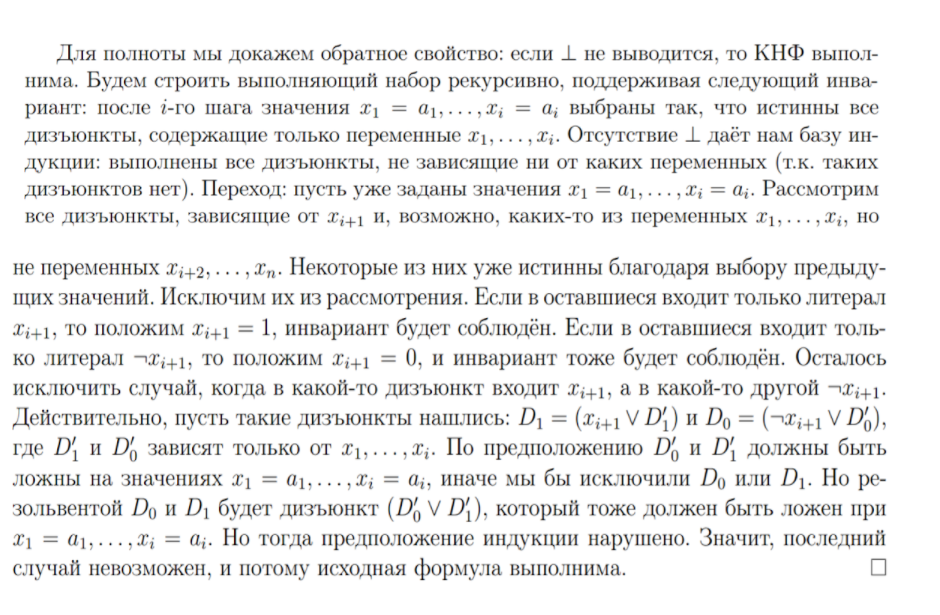
\includegraphics[width=0.9\textwidth]{images/1.4}

\newpage
\section{Задача Коши.}

\subsection{Принцип сжимающих отображений.}
\Def \textit{Линейное пространство} $L$ называется нормированным, если каждому его элементу $x$ поставлено в соответствие неотрицательное действительное число, называемое \textit{нормой} $x$ (обзначается $||x||$), обладающее свойствами:

1) $||x|| \geq 0, ||x|| = 0 \Longleftrightarrow x = 0_L$;

2) для любого $x \in L$ и $\lambda \in \R$ верно: $||\lambda x|| = |\lambda|\cdot ||x||$;

3) для любых $x, y \in L \quad ||x + y||\; \leqslant ||x|| + ||y||$.
\bigbreak
\noindent \Def Последовательность $\{ x_n \} \subset L$ называется \textit{сходящейся к $x \in L$ \underline{по норме}}, если \\ $\lim \limits_{n \rightarrow \infty} ||x_n - x|| = 0$.
\\
\Def Последовательность $\{ x_n \} \subset L$ называется \textit{фундаментальной} в норме, если \\ $||x_n - x_k|| \rightarrow 0$ при $n,k \rightarrow \infty$.
\bigbreak
\noindent
\Def Нормы $||\cdot||_1$ и $||\cdot||_2$ одного и того же нормированного пространства $L$ \textit{эквивалентны}, если $\exists c_1, c_2 > 0$, такие что $\forall x \in L \;\; c_1 {||x||}_2 \leqslant {||x||}_1 \leqslant c_2 {||x||}_2$.
\\
\Example Пространство функций, непрерывных на $[a, b]$, является линейным. Введём
две нормы:
\begin{equation*}
    ||f||_c = \sup_{x\in[a,b]}|f(x)|\ \text{(цэ-норма)},\\
    ||f||_{L_1} = \frac{1}{b - a} \int_a^b |f(x)|dx\ \text{($L_1$ норма)}.
\end{equation*}
Отметим, что равномерная сходимость является сходимостью по первой норме (цэ-норме), причём предел также непрерывен, а значит, принадлежит пространству.
\bigbreak
\noindent \Def Нормированное пространство, в котором каждая фундаментальная последовательность является сходящейся, является \textit{полным}. Но! Не во всяком нормированном пространстве фундаментальная последовательность сходится.
\\
\Def Полное линейное нормированное пространство называется \textit{банаховым}.
\\
\Def Открытый шар: $U_\varepsilon(a) = \{x \in L \;:\; ||x - a|| \,< \varepsilon\}$. Замкнутый: $\overline{U}_\varepsilon(a) =
\{\ldots \leqslant \varepsilon\}$
\bigbreak
Пусть $L_1$ и $L_2$ — банаховы пространства, $X\subseteq L_1$.
\\
\Def Оператор $\Phi: X \rightarrow L_2$ называется \textit{непрерывным} в точке $x_0$, если \\
\[\forall\varepsilon > 0 \;\; \exists\delta=\delta_{\varepsilon} \;\; \forall x \in U_\delta (x_0) \cap X \;\Rightarrow\; {||\Phi(x) - \Phi(x_0)||_2} < \varepsilon.\]
\bigbreak
Переходим в ситуацию, где $L_2 \equiv L_1$.
\\
\Def Точка $x^* \in X$ называется \textit{неподвижной точкой отображения} $\Phi$, если $\Phi(x^*) = x^*$.
\\
\Def Оператор $\Phi$ называется \textit{сжимающим на множестве $X$}, если $\exists q \in (0;1)$, такое что $\forall x_1, x_2 \in X \; \mapsto \; ||\Phi(x_1) - \Phi(x_2)|| \leqslant q||x_1 - x_2||$. Число $q$ — коэффициент сжатия.
\\
\Statement Сжимающее отображение является непрерывным:
\begin{equation*}
    \forall \varepsilon > 0 \;\; \exists \delta \leqslant \frac{\varepsilon}{q} \;\; \forall x_1,x_2 \; : \; x_1 \neq x_2 \mapsto ||x_1-x_2|| \;< \delta \quad \Rightarrow \quad ||\Phi(x_1)-\Phi(x_2)|| \;\leqslant q||x_1 - x_2|| \;\leqslant \varepsilon 
\end{equation*}

\subsection*{Теорема Банаха о неподвижной точке (принцип сжимающих отображений)}

Пусть $\Phi \,:\; \overline{U}_r (x_0) \to L$, причем $\Phi$ является сжимающим на $\overline{U}_r (x_0)$ с некоторым коэффициентом $q$. Тогда если выполнено условие $||\Phi(x_0) - x_0|| \leqslant (1-q)r$, то  в $\overline{U}_r (x_0)$ существует единственная неподвижная точка отображения.

\Proof Покажем, что $\Phi(\overline{U}_r(x_0))\subseteq\overline{U}_r(x_0)$. Пусть $x\in\overline{U}_r(x_0)$. Тогда 
\begin{equation*}
    ||\Phi(x) - x_0||\; = ||\Phi(x) -\Phi(x_0) + \Phi(x_0) - x_0||\; \leqslant ||\Phi(x) -\Phi(x_0)||\; +\; ||\Phi(x_0) - x_0||\; \leqslant
\end{equation*}
Так как отображение сжимающие, оценим первый модуль. Дополнительное условие в теореме используем для второго модуля.
\begin{equation*}
    \leqslant q||x - x_0|| \;+\; (1-q)\cdot r \leqslant q\cdot r + (1-q)\cdot r = r \qquad \Rightarrow \; \forall x \in \overline{U}_r(x_0) \;\; \Phi(x)\subseteq\overline{U}_r(x_0)
\end{equation*}
Рассмотрим последовательность $\{x_n\}\in\overline{U}_r(x_0)$, такую что $x_n = \Phi(x_{n-1})$ при $n \geqslant 1$. Также для удобства обозначим $\rho = ||\Phi(x_0) - x_0|| = ||x_1 - x_0||$. Покажем, что эта последовательность фундаментальная:
\begin{align*}
    ||x_2 - x_1|| \;= ||\Phi(x_1) - \Phi(x_0)||\; \leqslant q||x_1 - x_0||\; = q \cdot\rho \qquad \Rightarrow \;\ldots \; \Rightarrow\qquad
    ||x_{n+1} - x_n|| \;\leqslant q^n \rho
\end{align*}

Используем полученную оценку для того, чтобы оценить модули в сумме:
\begin{align*}
    \forall p \;\; ||x_{n+p} - x_n||\; \leqslant ||x_{n+p} - x_{n+p-1}|| \;+\; ||x_{n+p-1} - x_{n+p-2}|| \;+ \;\ldots + ||x_{n+1} - x_n||\; \leqslant \\ 
    \leqslant \rho (q^{n+p-1} + q^{n+p-2} + \dots + q^n) = \rho q^n (q^{p-1} + q^{p-2} + \dots + 1) = \frac{\rho q^n(1-q^p)}{1-q} < \frac{\rho q^n}{1 - q} \xrightarrow[n\to\infty]{}0
\end{align*}
А так как мы в банаховом пространстве (т.е. полном), то из фундаментальности получили сходящуюся последовательность.

$\exists \;x^* = \lim \limits_{n \rightarrow \infty} x_n$. А так как $\overline{U}_r (x_0)$ -- замкнутый шар, значит $x^* \in \overline{U}_r (x_0)$.
\\
Докажем, что $x^*$ является неподвижной точкой нашего оператора $\Phi$. Воспользуемся тем, что сжимающее отображение является неприрывным.

В $x_n = \Phi(x_{n-1})$ перейдём к пределу: $x^* = \lim \limits_{n \rightarrow \infty} x_n = \Phi(\lim \limits_{n \rightarrow \infty} x_{n-1}) = \Phi(x^*)$.
\\
Докажем единственность неподвижной точки.
Допустим, что существует $x^{**} \in \overline{U}_r (x_0): x^{**}= \Phi(x^{**})$, такое что $x^* \neq x^{**}$.

Тогда $||{x^* - x^{**}}|| \;=||\Phi(x^*) - \Phi(x^{**})|| \;\leqslant q\cdot ||x^* - x^{**}||$, где $q<1$, и получаем противоречие. \EndProof



\newpage

\subsection{Теоремы существования и единственности решения задачи Коши для нормальной системы дифференциальных уравнений и для уравнения \texorpdfstring{$n$}-го порядка в нормальном виде}
\setcounter{equation}{0}

\textbf{Определение} 
Пусть $n\geqslant 2$, $f_1,\ldots,f_n$ -- непрервные функции, определенные на $G \subseteq \R_{(x, \vec{y})}^{n+1}$. 
\newline Назовём \textit{нормальной системой дифференциальных уравнений первого порядка} следующую систему
\begin{equation}\label{Koshi1}
    \begin{cases}
    y_1'(x) = f_1(x, y_1(x), \dots, y_n(x)) = f_1 (x; \vec{y}(x)) \\
    \vdots \qquad \vdots \\
    y_n'(x) = f_n(x, y_1(x), \dots, y_n(x)) = f_n (x; \vec{y}(x)) \\
\end{cases}
\end{equation}
\begin{equation*}
    \text{Векторная форма: $\vec{y'} = \vec{f}(x; \vec{y})$, где $\vec{y}(x) = \left( \begin{matrix} y_1(x), \ldots, y_n(x) \end{matrix} \right)^T$}
\end{equation*}

\Def Вектор-функция $\vec{\varphi}(x)$ называется \textit{решением нормальной системы (\ref{Koshi1})} на некотором промежутке $I \subseteq \R$, если:

\begin{enumerate}
    \item $\vec{\varphi} (x) \in C^1(I)$
    \item $\forall x \in I \quad (x; \vec{\varphi}(x)) \in G$
    \item $\forall x \in I \quad \vec{\varphi'}(x) = f(x; \vec{\varphi}(x))$
\end{enumerate}
График решения $\vec{\varphi}(x)$ в пространстве $\R^{n+1}$ -- это интегральная кривая.
\bigbreak
\Def \textit{Задача Коши} -- это \begin{equation}\label{Koshi2}
    \begin{cases}
    \text{$\vec{y'} = \vec{f}(x; \vec{y})$ \;--\; нормальная система уравнений I-го порядка} \\
    \text{$\vec{y}(x_0) = \vec{y_0}$ \;\;\;--\; начальное условие} 
    \end{cases}
\end{equation}
Рассмотрим уравнение $\vec{y'} = f(x; \vec{y})$. Проинтегрируем его покомпонентно. Получим слева искомое $y(x)$, справа ищем одну из первообразных как интеграл с переменным верхним пределом: 
\begin{equation}\label{Koshi3}
    y(x) = \int \limits_{x_0}^{x} f(\tau ; \vec{y}(\tau))d\tau + \vec{y_0}
\end{equation}
\par \Def Вектор-функция $\vec{\varphi}(x)$ из пространства $C_n(I)$ называется \textit{решением интегрального уравнения (\ref{Koshi3})} на $I\subseteq\R$, если:

\begin{enumerate}
    \item $\vec{\varphi}(x) \in C^1(I)$
    \item $\forall x \in I \quad (x; \vec{\varphi}(x)) \in G$
    \item $\forall x \in I \quad \vec{\varphi}(x) = \int \limits_{x_0}^x f(\tau; \vec{y}(\tau))d\tau + \vec{y_0}$
\end{enumerate}

\Lemma (об эквивалентности) Вектор-функция $\vec{\varphi}(x)$ является решением задачи Коши (\ref{Koshi2}) на $I$ тогда и только тогда, когда $\vec{\varphi}(x)$ на том же $I$ является решением (\ref{Koshi3}).

\Proof

\fbox{$\Longrightarrow$} Пусть $\vec{y}=\vec{\varphi}(x)$ -- решение ЗК на $I$. Тогда $\vec{y'}(x) = f(x; \vec{y}(x))$, значит, $\vec{y}(x) = \int \limits_{x_0}^{x} \vec{f}(\tau; \vec{y}(\tau))d\tau + C$. Из начального условия $y_0 = \vec{y}(x_0) = \int \limits_{x_0}^x \dots d\tau + C \;\;\Rightarrow\;\; C = \vec{y_0} \;\;\Rightarrow\;\; \vec{y}(x) = \int \limits_{x_0}^{x} \vec{f}(\tau; \vec{y}(\tau))d\tau + \vec{y_0}$.

\fbox{$\Longleftarrow$} Пусть $\vec{y}=\vec{\varphi}(x)$ -- решение интегрального уравнения. $\forall x \in I$ $\vec{\varphi}(x) = 
\int \limits_{x_0}^{x} \vec{f}(\tau; \vec{\varphi}(\tau))d\tau + \vec{y_0}$.
\newline Дифференцируем по $x$, получим 
\(\vec{\varphi'} = \vec{f}(x;\vec{\varphi}(x))\) \;и\; 
\(\vec{\varphi}(x_0) = \int \limits_{x_0}^{x_0} \dots d\tau + \vec{y_0} = \vec{y_0}\). \quad \EndProof


Возьмём кубическую норму: $|\vec{y}| = \max \limits_{1 \leqslant i \leqslant n} |y_i|$
\\
\Def Вектор-функция $\vec{f}(x; \vec{y})$, определённая в области $G \subseteq \R_{(x, \vec{y})}^{n + 1}$ называется \textit{удовлетворяющей условию Липшица} относительно $\vec{y}$ равномерно по $x$, если $\exists L > 0$ такой, что $\forall (x; \vec{y_1})$ и $(x; \vec{y_2})$ верно, что $|\vec{f}(x; \vec{y_1}) - \vec{f}(x; \vec{y_2})|\; \leqslant L|\vec{y_1} - \vec{y_2}|$.
\bigbreak
\Lemma Вектор-функция $\vec{f}(x; \vec{y})$ удовлетворяет условию Липшица по $\vec{y}$ равномерно по $x$ при выполнении следующих условий:

\begin{enumerate}
    \item $G$ -- выпуклая область в $\R^{n + 1}$;
    \item $\vec{f} (x; \vec{y}) \in C_n(G)$, т.е. непрерывна (от $n$ аргументов) и $\forall i, j = \overline{1,n}$\; $\frac{\partial f_i}{\partial y_j} \in C(G)$
    \item $\exists K > 0:$ $\forall i, j = \overline{1,n}$ \; $\forall (x, \vec{y}) \in G:\;$ $|\frac{\partial \vec{f}_i}{\partial y_i} (x; \vec{y})| \leqslant K$.
\end{enumerate}

\Proof Фиксируем $i = 1, \dots, n$. Рассмотрим $(x; \vec{y_1})$, где $\vec{y_1} = (y_{1_1}, \dots, y_{1_n})$, а также $\vec{y_2} = (y_{2_1}, \dots, y_{2_n})$.
\begin{align*}
    |f_i (x; \vec{y_1}) - f_i (x; \vec{y_2})| \,= \Big|f_i (x; \vec{y_2} + \theta(\vec{y_1} - \vec{y_2}))|_{\theta = 0}^{\theta = 1}\Big| \stackrel{\footnotesize{\text{Ньютон-Лейбниц}}}{=} \bigg| \int \limits_0^1 \Big[\frac{d}{d \theta} f_i (x; \vec{y_2} + \theta (\vec{y_1} - \vec{y_2})) \Big]d \theta\bigg| = \\
    = \bigg|\int \limits_0^1 \sum \limits_{j = 1}^n \frac{\partial f_i (x; \vec{y_2} +  \theta(\vec{y_1} - \vec{y_2}))}{\partial y_j}(y_{1_j} - y_{2_j}) d\theta\bigg| \; \leqslant \sum \limits_{j = 1}^{n} \int \limits_0^1 \underbrace{\bigg|\frac{\partial f_i (x; \vec{y_2} +  \theta(\vec{y_1} - \vec{y_2}))}{\partial y_j}\bigg|}_{\leqslant K}\cdot \underbrace{|y_{1_j} - y_{2_j}|}_{\leqslant |\vec{y_1} - \vec{y_2}|} d\theta \leqslant \\
    \leqslant \underbrace{n\cdot K}_{=L} \cdot |\vec{y_1} - \vec{y_2}| \qquad \Rightarrow \qquad |\vec{f}(x; \vec{y_1}) - \vec{f}(x; \vec{y_2})| = \max \limits_{1 \leqslant i \leqslant n} |f_i (x; \vec{y_1}) - f_i  (x; \vec{y_2})| \leqslant L \cdot |\vec{y_1} - \vec{y_2}| \quad \text{\EndProof }
\end{align*}

\subsection*{Теорема о существовании и единственности решения задачи Коши для системы уравнений $n$-го порядка в нормальном форме}

\noindent Пусть вектор-функция $\vec{f} \brackets{x, \vec{y}}$ непрерывна в области $G$ вместе со своими производными по $y_j \;(j = \overline{1, n})$, точка $(x_0, \vec{y_0})$ тоже лежит в $G$. Тогда задача Коши локально разрешима единственным образом:

\begin{enumerate}
    \item \(\exists \delta > 0\), такое что на $[x_0 - \delta, x_0 + \delta]$ решение задачи Коши существует;
    \item Решение единственно в следующем смысле: \\
    Если $\vec{y_1} (x) \equiv \vec{\varphi}(x)$ — решение задачи Коши в $\delta_1$-окрестности точки $x_0$, а $\vec{y_2} \equiv \vec{\psi}(x)$ — решение задачи Коши в $\delta_2$-окрестности точки $x_0$, то в окрестности точки $x_0$ с радиусом $\delta = \min (\delta_1, \delta_2)\newline \vec{\varphi}(x) \equiv \vec{\psi}(x)$. 
\end{enumerate}

\noindent \Proof Рассмотрим множество $\overline{H_{\delta, r}} (x_0) = \{ (x, \vec{y}) \in G: x \in [x_0 - \delta, x_0 + \delta] \;\; \text{и} \;\; |\vec{y} - \vec{y_0}| \leqslant r \} \subset G$. \newline Заметим, что в силу компактности этого множества (что следует из ограниченности и замкнутости) применима теорема Вейерштрасса (непрерывная на компакте функция ограничена): $\exists M > 0: \forall (x, \vec{y}) \in \overline{H_{\delta, r}} \;\; |\vec{f} (x, \vec{y})| \leqslant M$ \; и \; $\forall i, j =  \overline{1, n}$\;\; $\Big|\mathlarger{\frac{\partial f_i}{\partial y_j}}\Big| \leqslant M$. \newline Значит, $\vec{f}(x, \vec{y})$ на $\overline{H_{\delta, r}} (x_0)$ удовлетворяет условию Липшица относительно $\vec{y}$ равномерно по $x$. \newline Рассмотрим интегральное уравнение, которое как мы доказали ранее эквивалетно ЗК:

\begin{equation*}
    \vec{y}(x) = \vec{y_0} + \int \limits_{x_0}^x \vec{f}\brackets{\tau, \vec{y}(\tau)} d\tau \;\;\Longleftrightarrow \;\;\vec{y} = \Phi(\vec{y})
\end{equation*}

Рассмотрим в $C_n [x_0 - \delta, x_0 + \delta]$ замкнутый шар $\overline{D_{\delta, r}}(\vec{y_0}) = \{ \vec{y} \in C_n [x_0 - \delta, x_0 + \delta]: {||\vec{y} - \vec{y_0}||}_{C_n} \leqslant r \}$, где ${||\vec{y}||}_{C_n} = \max \limits_{1 \leqslant i \leqslant n} \sup \limits_{|x - x_0| < \delta} |y_i (x)|$. 

\noindent Докажем, что существуют $\delta$ и $r$ такие, что 
\begin{itemize}
    \item $\Phi$ является сжимающим
    \item отображает шар $\overline{D_{\delta, r}} (\vec{y_0})$ в себя 
\end{itemize}
Тогда мы сможем применить теорему Банаха о сжимающем отображении. Получим единственную неподвижную точку отображения $\Leftrightarrow$ интегральное уравнение имеет единственное решение $\Leftrightarrow$ ЗК имеет единственное решение.
\bigbreak
Докажем, что $\Phi$ является сжимающим. Рассмотрим $\vec{y}, \vec{z} \in \overline{D_{\delta, r}} (\vec{y_0})$ (функции): 
\begin{align*}
    ||\Phi(\vec{y}) - \Phi(\vec{z})|| \; &= \max \limits_{i = 1, \dots, n} \sup \limits_{|x - x_0| \leqslant \delta} \bigg|\int \limits_{x_0}^{x} \brackets{f_i(\tau, \vec{y}(\tau)) - f_i (\tau, \vec{z}(\tau))}d\tau\bigg| \; \leqslant \\
    &\leqslant \max \limits_{i = 1, \dots, n} \sup \limits_{|x - x_0| < \delta} \int \limits_{x_0}^x \underbrace{\Big|f_i(\tau, \vec{y}(\tau)) - f_i (\tau, \vec{z}(\tau))\Big|}_{\mathlarger{\leqslant |\vec{f}(\tau; \vec{y}) - \vec{f}(\tau; \vec{z})|}} d\tau \leqslant \\
    &\leqslant \sup \limits_{|x - x_0| < \delta} \int \limits_{x_0}^{x} L |\vec{y}(\tau) - \vec{z}(\tau)|d\tau \;\leqslant\; \sup \limits_{|x - x_0| < \delta} \int \limits_{x_0}^{x} L ||\vec{y} - \vec{z}||_{C_n} d\tau \; \leqslant \; \underbrace{\delta L}_{=q < 1} {||\vec{y} - \vec{z}||}_{C_n}
\end{align*}
Положим $\delta = \frac{q}{L}$, получим требуемое.
\bigbreak
Теперь докажем вторую часть:
\begin{align*}
    ||\Phi(\vec{y_0}) - \vec{y_0}|| = \max \limits_{i = 1, \dots, n} \sup \limits_{|x - x_0| < \delta} \bigg|\int \limits_{x_0}^x f_i \brackets{\tau, \vec{y_0}} d\tau\bigg|
    \leqslant \int \limits_{x_0}^x \brackets{\max \limits_{i = 1, \dots, n} \sup \limits_{|x - x_0| < \delta} |f_i (\tau, \vec{y_0})| d\tau} = \\
    = \int \limits_{x_0}^{x} {||\vec{f}(\tau, \vec{y_0})||}_{C_n} d\tau \;\leqslant \; \delta M = (1 - q) r
\end{align*}

Получили, что $\begin{cases} q = \delta L \\ (1 - q)r = \delta M \end{cases} \Longrightarrow \;\; \begin{cases} r - rq = \delta M \\ r = \delta L r + \delta M \end{cases} \Longrightarrow  \;\;\delta_r = \mathlarger{\frac{r}{M + Lr}}$ \qquad \EndProof

\subsection*{Теорема о существовании и единственности решения задачи Коши для уравнения $n$-го порядка в нормальном виде}

\noindent Нормальный вид -- уравнение разрешённо относительно старшей производной

\begin{equation*}
    \begin{cases}
    y^{(n)}=f(x,y,y',\ldots,y^{(n-1)}) \\
    y(x_0) = y_0\\
    y'(x_0) = y_0^1\\
    \ldots\\
    y^{(n-1)}(x_0)=y_0^{(n-1)}
    \end{cases}
\end{equation*}

Пусть функция $f(x, y, p_1, \ldots , p_{n-1})$ определена и непрерывна по совокупности переменных
вместе с частными производными по переменным $y, p_1, \ldots , p_{n-1}$ в некоторой области $G \subseteq \R^{n+1}$, и точка $(x_0, y_0, y^1_0, \ldots , y^{n-1}_0) \in G$, тогда существует замкнутая $\delta$-окрестность точки $x_0$, в
которой существует единственное (в ранее указанном смысле) решение задачи Коши.

\Proof Пусть $\vec{z} = (y,y',\ldots,y^{(n-1)})^T$ -- вектор-функция. Запишем: 
\begin{figure}[h]
    \vspace{-4ex}
    \hspace{-4ex} \begin{minipage}[h]{0.4\linewidth}
        \begin{align*}
            z_1'=z_2 \\
            z_2'=z_3 \\
            \ldots \\
            z_{n-1}'=z_n \\
            z_n'=f(x,z_1,z_2,\ldots,z_n)=f(x,\vec{z})
        \end{align*}
    \end{minipage}
    \hfill
    \hspace{-4ex} \begin{minipage}[h]{0.6\linewidth}
    Введём обозначение: $\vec{g}(x,\vec{z})=(z_2,z_3,\ldots,z_n, f(x,\vec{z}))^T$.
    \\
    Перепишем задачу Коши: $
        \begin{cases}
        \vec{z'}=\vec{g}(x,\vec{z}) \\
        \vec{z}(x_0)=\vec{z_0}
        \end{cases}
    $
    \end{minipage}
\end{figure}

\noindent Согласно предыдущей теореме, существует единственное решение полученной задачи
Коши в некоторой замкнутой $\delta$-окрестности точки $x_0$; эта же окрестность подходит и для
исходной ЗК. \; \EndProof
\bigbreak
Интегральная кривая для данной задачи определяется как множество точек вида:
$$\Big(x, y(x), y'(x), \ldots,y^{(n-1)}(x)\Big)$$

\newpage

\subsection{Теоремы о продолжении решения для нормальной системы дифференциальных уравнений}
\subsection{Теорема о структуре вполне упорядоченного множество: оно представляется как $\omega \cdot L + F$, где $L$ — множество предельных элементов (кроме, возможно, наибольшего), $F$ — конечное множество.}

\par $\blacktriangle$ Пусть $P$ - множество предельных элементов нашего ВУМа. Заметим, что $P$ - ВУМ (как подмножество ВУМа). Рассмотрим элемент $x \in P$. Пусть $Sx=y$ (следующий элемент). Построим биекцию между $\omega$ и $[x; y)$. Числу $n$ из $\omega$ поставим в соответствие число $\underbrace{SS\ldots S}_\text{$n$ раз}x$. Очевидно, что это инъекция ($x+n=x+m \Leftrightarrow n=m$).
\par Докажем, что это сюръекция. Рассмотрим элемент $t$ лежащий в $[x;y)$. Бесконечно уменьшать его на 1 (то есть брать предыдущий) нельзя по одному из эквивалентных определений фундированности $\Rightarrow$ существует предельный элемент $k$ (у которого нет предыдущего), такой что  $S\ldots Sk=t$. $k$ лежит на в $[x,y)$, но единственный предельный элемент, лежащий в этом множестве - это $x \Rightarrow k=x \Rightarrow t=S\ldots Sk$ будет получен. 
\par Повторим такие действия для всех $x$ (кроме наибольшего). Затем возможны 2 случая
\begin{enumerate}
    \item В исходном ВУМе нет наибольшего элемента. Тогда аналогично прошлым шагам строим изоморфизм между $\omega$ и оставшимися элементами. Получаем, что наш ВУМ равен $\omega \cdot P$
    \item В исходном ВУМе есть наибольший элемент. Тогда осталось лишь конечное число нерассмотренных элементов. Докажем это
    \par Обозначим наибольший элемент всего ВУМа как $a$. По определению фундированности, мы не сможем бесконечно брать предыдущий элемент $\Rightarrow$ существует $k$ - предельный, такой что $a=\underbrace{S\ldots S}_\text{$m$ раз}k$. $k \geq x,$ но $x$ - наибольший из предельных элементов $\Rightarrow$ $k=x \Rightarrow |[x;a]|=m+1$. Построим биекцию между этим отрезком и множеством $F=[0;m]$.
\end{enumerate}

\par Таким образом, получаем, что наше ВУМ равномощно $\omega \cdot L + F$, где $L$ - множество предельных элементов кроме, возможно, наибольшего, а $F$ - конечное множество $\blacksquare$
\newpage

\subsection{Непрерывная зависимость от параметров решения задачи Коши для нормальной системы дифференциальных уравнений (б/д)}
Дифференциальные уравнения, описывающие физические
процессы, всегда содержат некоторые параметры (масса,
упругость и т.д.). Эти параметры в реальных задачах
никогда не могут быть измерены абсолютно точно, т.е.
всегда измеряются с некоторой погрешностью, так что
сами дифференциальные уравнения известны лишь с некоторой степенью точности. Поэтому, для того чтобы
уравнения могли описывать реальные процессы, необходимо, чтобы их решения непрерывно зависели от параметров, т.е. чтобы они мало менялись при малых изменениях параметров.
\bigbreak
Рассмотрим задачу Коши для нормальной системы дифференциальных уравнений в векторном виде т.е. $ \vec{f}=(f_1,\ldots,f_n)$:
\setcounter{equation}{0}
\begin{equation}\label{eq_0}
    \frac{d\vec{y}}{dx}=\vec{f}(x,\vec{y},\vec{\mu}), \qquad \vec{y}(x_0,\vec{\mu})=\vec{y_0}(\vec{\mu})
\end{equation}
где $\mu$ -- параметр, $\mu_0$ -- задан.
\bigbreak
\par \Th  Пусть $\vec{f}(x,\vec{y},\vec{\mu})$ -- непрерывна и удовлетворяет условию Липшица равномерно по $x$ и $\vec{\mu}$, $\forall (x,\vec{y}) \in G \subseteq \R^{n+1}$ и всех $\vec{\mu}$, таких что $|\vec{\mu} - \vec{\mu}_0| \leqslant \delta$. Пусть кроме того, $(x_0,\vec{y_0}) \in G$. \newline Тогда $\exists h > 0 \;\mapsto$ решение $\vec{y}(x,\vec{\mu})$ задачи Коши (\ref{eq_0}) непрерывно по совокупности переменных $(x,\vec{\mu})$ в некоторой области $|x-x_0|\leqslant h$, $|\vec{\mu}-\vec{\mu}_0|\leqslant \delta$.
\bigbreak
\Note Интегральные кривые уравнения в этой теореме образуют семейство кривых, проходящих через точку $(x_0,\vec{y_0})$. Теорема утверждает, что интегральные кривые, отвечающие близким значениям параметра $\vec{\mu}$, близки.
\bigbreak
\bigbreak
\subsection{Дифференцируемость решения по параметрам, уравнение в вариациях (б/д)}
\Th Если при $(x,y)\in G$ и $|\vec{\mu} - \vec{\mu}_0| \leqslant \delta$ функции \[f(x,y,\vec{\mu}) \qquad \frac{\partial f}{\partial y} \qquad \frac{\partial f}{\partial \mu_i}\]
непрерывны, а также $(x_0,y_0)\in G$, то $\exists h > 0 \;\mapsto$, что при  $|x-x_0|\leqslant h$, $|\vec{\mu}-\vec{\mu}_0|\leqslant \delta$ для решения $y = \varphi(x,\vec{\mu})$ задачи Коши (\ref{eq_0}) верно следующее:
\begin{enumerate}
    \item $z_i(x,\vec{\mu}) = \mathlarger{\frac{\partial \varphi}{\partial\mu_i}}$ непрерывны для указанных $x$ и $\vec{\mu}$
    \item  Смешанные производные $\mathlarger{\frac{\partial^2\varphi}{\partial x \partial \mu_i}}$ непрерывны и не зависят от порядка дифференцирования
    \item  Частные производные $z_i$ удовлетворяют уравнениям в вариациях по параметру $\vec{\mu}$:
    \begin{equation}\label{eq_1}
    \frac{\partial z_i}{\partial x}= \frac{\partial f(x, \varphi(x, \vec{\mu}), \vec{\mu})}{\partial y}\cdot z_i + \frac{\partial f(x, \varphi(x, \vec{\mu}), \vec{\mu})}{\partial\mu_i}
    \end{equation}
    и  начальным условиям $z_i(x_0,\vec{\mu}) = 0$.
\end{enumerate}

\Def Если обе части уравнения (\ref{eq_1}) продифференцировать по $\mu_i$, то получим уравнение, которое называется \textit{уравнением в вариациях}.

\Note Уравнение в вариациях всегда линейное.
\newpage

\subsection{Задача Коши для уравнения первого порядка, не разрешенного относительно производной, теорема существования и единственности решения задачи Коши.}
\label{zk-notsolved}
Путь у нас есть задача Коши
\begin{center}
    $\begin{cases}
    F \brackets{x, y, y'} = 0; \\
    y\brackets{x_0} = y_0; \\
    y'\brackets{x_0} = p_0
    \end{cases}$
\end{center}

\textbf{Теорема($\exists ! \text{решение ЗК для ур-ния 1-го порядка, не разр. отн. } y'$):}
\newline Пусть $F(x, y, p)$ опрелена и непреывна вместе с $ \frac{\del F}{\del y} $ и $ \frac{\del F}{\del p} $ в некоторой области $G\subseteq \R^3$ и в точке $(x_0, y_0, p_0) \in G $ справедливо $\mathlarger{\frac{\del F}{\del p} \bigg|_{\brackets{x_0, y_0, p_0}}}\!\!\! \neq 0$. \newline Тогда существует $\delta > 0$, такое что на отрезке $[x_0 - \delta; x_0 + \delta]$ существует и единственно решение ЗК. 
\bigbreak
\Proof Так как $\frac{\del F}{\del p} \neq 0$ и частные производные непрерывны в $G$, то по теореме о неявной функции существует окрестность точки $\brackets{x_0, y_0}$ и существует непрерывно дифференцируемая функция $f\brackets{x,y}$, определённая на окрестности $(x_0, y_0)$, такая что $f\brackets{x_0, y_0} = p_0$ и для любой точки из $(x_0, y_0)$ верно равенство $p = f(x, y)$. Тогда задача Коши будет формулироваться так:

\begin{center}
    $\begin{cases}
    y' = f\brackets{x, y}; \\
    y\brackets{x_0} = y_0
    \end{cases}$
\end{center}

Вновь применим теорему о неявной функции, получим $\mathlarger{\frac{\del f}{\del y} = - \frac{\frac{\del F}{\del y} \brackets{x, y, p}}{\frac{\del F}{\del p} \brackets{x, y, p}} \bigg|_{p = f \brackets{x, y}}}$.

Внутри окрестности точки $(x_0, y_0)$ можно взять выпуклую область, на которой для $f(x,y)$ будет выполняться условие Липшица. Тогда получим требуемое по теореме о существовании и единственности решения задачи Коши для уравнения, разрешённого относительно производной. \EndProof

\subsection{Особые решения}
\subsection{Теорема о делении с остатком вполне упорядоченных множеств.}

\textbf{Теорема} $\forall \alpha, \beta \quad \exists ! \gamma, \delta : \delta < \alpha$ и $\alpha = \beta \cdot \gamma + \delta$, где $\alpha, \beta, \gamma, \delta$ -- ВУМы.\\

\textbf{Доказательство:}\\

1) Существование.

Рассмотрим $\zeta$ такое, что заведомо $\beta \zeta > \alpha$ (например, подойдет $\zeta = \alpha + 1$).\\

Это значит, что $\alpha$ равняется некоторому начальному отрезку $\beta \zeta$. Этот начальный отрезок представляется в виде $[0;q), q \in \beta \zeta$ и потому $q = (b, g), b \in \beta, g \in \zeta$\\

$\alpha \in [0;q) \Rightarrow \alpha = (s, t) :$ либо $t < g$, а $s$ любое из $\beta$, либо $t = g, s < b$.\\

Для каждого $t < g$ получаем экземпляр $\beta$, порядок на этих экземплярах взят с $[0;g)$

В итоге : $\gamma = [0;g), \delta = [0;b)$\\

2) Единственность.

Если $\gamma_1 = \gamma_2,$ то аналогично единственности вычитания.
Если $\gamma_1 < \gamma_2$, то $\gamma_1 + 1 \leq \gamma_2$ и поэтому $\beta \cdot \gamma_1 + \delta_1 < \beta \cdot \gamma_1 + \beta = \beta \cdot (\gamma_1 + 1) \leq \beta \cdot \gamma_2 \leq \beta \cdot \gamma_2 + \delta_2$.
\newpage

\section{Линейные дифференциальные уравнения и линейные системы дифференциальных уравнений с постоянными коэффициентами}

\subsection{Фундаментальная система решений и общее решение линейного однородного уравнения n-го порядка}
\label{firstthird-anchor}
\subsection{Эквивалентность следующих утверждений: множество перечислимо, полухарактеристическая функция множества вычислима, множество является областью
определения вычислимой функции, множество является проекцией разрешимого
множества пар.}

\textbf{Теорема.} Следующие утверждения для непустого $S \subseteq \mathbb{N}$ эквивалентны:

1) S перечислимо (существует печатающая машина, такая, что $\forall x \in S$ x встречается в потоке вывода, $\forall x \notin S$ x не встречается в потоке вывода);

2) Полухарактеристическая функция множества (равная 0 на элементах S и не определённая вне S) вычислима;

3) S - область определения вычислимой функции (если существует алгоритм, её вычисляющий, то
есть такой алгоритм A, что $\forall f(n)$ определённых для некоторого n алгоритм А остановится на входе n и напечатает f(n), иначе - не остановится на входе n);

4) S - проекция разрешимого (существует алгоритм, который по любому натуральному n определяет, принадлежит ли оно множеству) множества пар.

$\blacktriangle$
(1) $\Rightarrow$ (2). Запускаем эту печатающую машину. Если она выдаёт x, то значение полухарактеристической функции 1, иначе - $\perp$.

(2) $\Rightarrow$ (3). S - область определения характеристической функции, описанной ранее.

(3) $\Rightarrow$ (1). Пусть S - область определения вычислимой функции f, вычисляемой алгоритмом B. Тогда есть алгоритм, перечисляющий A: параллельно запускать B на входах 0, 1, 2, ..., делая всё больше шагов (1 шаг на входах 0 и 1, 2 шага - на входах 0, 1, 2, и.т.д.); напечатать все номера, на которых B остановился. 

(1) $\Rightarrow$ (4). S = $\{ x | \exists n (x, n) \in B\}$ - проекция множества $B = \{ (x, n):$ x в первых n шагах алгоритма, перечисляющего S$\}$

(4) $\Rightarrow$ (1). for (x=0;; ++x) \\
for (y=0;; ++y) 

    $\{ if ((x, y) \in B)$ cout $<<$ x;

    $if ((y, x) \in B)$ cout $<<$ y; $\}$
$\blacksquare$

\newpage

\subsection{Линейное неоднородное уравнение \texorpdfstring{$n$}-го порядка с постоянными коэффициентами и правой частью квазимногочленом}
\Def Эти уравнения имеют вид
\[y^{(n)}+a_1y^{(n-1)}+a_2y^{(n-2)}+...+a_n y = f(x),\]
где $f(x)$ квазимногочлен: $f(x) = e^{\mu x} P_m(x)$, $\mu \in \mathbf{C}$ $P_m(x)$ - заданный многочлен степени $m$ с комплексными коэффициентами. 

\Def Характеристическим многочленом $L(x)$ назовём многочлен
\[L(X) = a_n x^n + a_{n-1} x^{n-1} + ... + a_0\]

\Def Дифференциальным оператором $D$ назовём оператор
\[D = \frac{d}{dx}\]

\Note $D^n y = y^{(n)}$ 

Существование и единственность решения следуют из таковых для системы

\begin{equation*}
    \begin{cases}
        \vec{y'}_1 = y_2&\\
        \vec{y'}_2 = y_3&\\
        \ldots&\\
        \vec{y'}_{n-1} = y_n&\\
        \vec{y'}_n = f - a_1 y_1 - a_{2}y_2 - \ldots - a_n y_n
    \end{cases}
\end{equation*}

(здесь $y_1 = y$)
\bigbreak
\Def Если число $\mu$ является корнем характеристического уравнения 
\[L(\lambda) = \lambda^n + a_1 \lambda^{n-1}+...+ a_n = 0\]
то говорят, что в уравнении резонансный случай. Если же $\mu$ не является корнем, то имеем нерезонансный случай.

\Def Дифференциальным многочленом назовём многочлен вида 
\[L(D) = (D-\lambda_1)^{k_1} (D-\lambda_2)^{k_2} ... (D-\lambda_s)^{k_s},\]
Где $k_s$ соответствующие кратности корней характеристического уравнения
\bigbreak
Рассмотрим ЛОУ. Покажем, что если известно некоторое решение $y_0(x)$ ЛНУ, то замена $y = z + y_0$ приводит уравнение к ЛОУ. Воспользуемся представлением левой части через дифференциальный многочлен:

\[L(D)y=L(D)(z+y_0) =L(D)z + L(D) y_0 = L(D)z + f(x) = f(x)\]

Откуда следует, что $L(D)z = 0$, т.е. решение.

Рассмотрим $L(D) y(x) = e^{\mu x} P_m(x)$.
\bigbreak
\Statement $(P_m(x)e^{\lambda x})'_x = Q_m(x)e^{\lambda x}$

\begin{theorem}[О структуре ФСР]
Пусть $\lambda_1, ..., \lambda_k$ корни характеристического многочлена кратности $l_1, ..., l_k$. Тогда набор функций $x^s e^{\lambda_i x}$, где $s = 0,..., l_1-1$, $i = 1, ..., k$ является ФСР для рассматриваемого уравнения
\end{theorem}
Доказано в пункте~<<\nameref{firstthird-anchor}>>.

\begin{theorem}[О структуре решения ЛНУ c правой частью в виде квазимногочлена]
Для рассматриваемого уравнения существует и единственно решение вида
\[y(x) = x^k e^{\mu x} Q_m(x) \]
где $ Q_m(x)$ - многочлен одинаковой с $P_m(x)$ степени $m$, а число $k$ равно кратности корня $\mu$ в уравнении $L(\lambda)=0$ в резонансном случае и $k=0$ в нерезонансном
\end{theorem}

\Proof
Если $\mu \neq 0$, то заменой $y = z e^{\mu x}$ всегда можно избавиться от $e^{\mu x}$ в правой части. В самом деле, по формуле сдвига после замены имеем что \[L(D) y = L(D)(e^{\mu x} z) = e^{\mu x} L(D+\mu) z = e^{\mu x}  P_m(x),\]
откуда $L(D+\mu)z=P_m(x)$.

Таким образом, доказательство теоремы осталось провести для уравнения вида
\[L(D)y=P_m(x)\]

\begin{enumerate}
    \item Нерезонансный случай: $L(\mu) \neq 0$. Пусть
    \[P_m(x) = p_m x^m + ... + p_0\]
    \[Q_m(x) = q_m x^m + ... + q_0\]
    Если подставить и приравнять коэффициенты при одинаковых степенях $x$, получим линейную алгебраическую систему уравнения для опредения неизвестных коэффициентов $q_0, ... q_m$. Матрица системы треугольная с числами $a_n = L(0) \neq 0$, таким образом, все коэффициенты определяются из неё одназначно.
    \item В резонансном случае имеем 
    \[L(\lambda) = \lambda^k (\lambda^{n-k} + a_1 \lambda^{n-k-1} + ...+a_{n-k}) \]
    Следовательно,
    \begin{equation*}
        L(D) = 
        \begin{cases}
           D^n + a_1 D^{n-1} + ... + a_{n-k} D^k, k < n\\
           D^n, k = n
        \end{cases}
    \end{equation*}
    В первом случае замена $D^k y = z$ приводит к уравнению с нерезонансным случаем. Рассмотрим уравнение
    \begin{equation*}
        D^k(y) = 
        \begin{cases}
           R_m(x), k < n\\
           P_m(x), k = n
        \end{cases}
    \end{equation*}
    Взяв нулевые начальные условия для этого уравнения
        \[y(x) = y'(0) = ... = y^{(k-1)} (0) = 0\]
        получим единственное решение вида 
    \[y(x) = x^k Q_m(x)\]
\end{enumerate}
\EndProof

\textbf{О вещественнозначной ФСР}
Для уравнения с вещественнозначными коэффициентами комплексные корни $M(\lambda)$ распадаются на сопряжённые пары одинаковой кратности. Соответствующие им решения легко
заменяются на вещественные функции (по аналогии с однократными действительными корнями $M(\lambda)$).


\newpage

\subsection{Уравнение Эйлера}
Уравнением Эйлера называется уравнение вида
\[
x^n y^{(n)} + a_1 x^{n-1} y^{(n-1)} + a_2 x^{n-2} y^{(n-2)} + ... + a_{n-1} x y^{'} + a_n y = 0
\]
Данное уравнение сводится к уравнению с постоянными коэффициентами при замене $x = e^t$ при $x > 0$ и  $x = -e^t$ при $x < 0$.
 
Докажем это индукцией по порядку:

\begin{align*}
    \frac{dy}{dx} &= \frac{y^{'}_t}{x^{'}_t} = e^{-t} y^{'}_t\\
    \frac{d^2 y}{dx^2} &= e^{-2t} ( y^{''}_t - y^{'}_t)\\
    \frac{d^3 y}{dx^3} &= e^{-3t} ( y^{'''}_t - 3y^{''}_t + 2 y^{'}_t)\\
    &\ldots\\
    \frac{d^n y}{dx^n} &=  e^{-nt} \varphi(y^{(n)}_t, y^{(n-1)}_t, \ldots, y^{'}_t)
\end{align*}

Подставим найденные выражения в определение и получим уравнение вида, где $y^{(n)}$ зависит от нового параметра $t$:

\[a_0 y^{(n)} + b_1 y^{(n-1)} + b_2 y^{(n-2)} + ... + b_{n-1} y^{'} + b_n y = 0\]

Поскольку мы получили линейное однородное с постоянными коэффициентами, то его фундаментальная система решений может содержать лишь функции вида

\[ e^{\lambda t}, \;  t^k e^{\lambda t}, \;  e^{\lambda t} cos(\gamma t), \;  e^{\lambda t} sin(\gamma t), \; 
 t^k e^{\lambda t}  cos(\gamma t), \; 
  t^k e^{\lambda t}  sin(\gamma t) \]
\newpage

\subsection{Фундаментальная система решений и общее решение нормальной линейной однородной системы уравнений}

\Def \textit{Нормальной системой дифференциальных уравнений} называется система дифференциальных уравнений первого порядка, разрешённых относительно производной:
\begin{equation*}
 \begin{cases}
   y_1' = f_1(x, y_1, ..., y_n) \\
   \dots \\
   y_n' = f_n(x, y_1, ..., y_n)
 \end{cases}
\end{equation*}
где $x$ -- независимая переменная,\\
$y_1(x), \dots, y_n(x)$ -- неизвестные функции


\textbf{Построение фундаментальной системы решений}

$$
\Vec{x}(t) = \begin{pmatrix}
x_{1}(t)\\
\vdots\\
x_{n}(t)
\end{pmatrix},\ \ \ 
A_{n\times n} = (a_{ij}),\ \ \ 
\Vec{f} = \begin{pmatrix}
f_{1}(t)\\
\vdots\\
f_{n}(t)
\end{pmatrix} 
$$
\begin{equation}
\dot{\Vec{x}} = A\Vec{x} + \Vec{f}(t)
\end{equation}

\begin{equation}\label{dotxax}
\dot{\Vec{x}} = A\Vec{x}
\end{equation}

\Th Если $\Vec{h_1}, \dots,\Vec{h_n}$ - базис из собственных векторов матрицы $A$, то $\Vec{x_i} = e^{\lambda_it}\Vec{h_i}$ - ФСР для уравнения (\ref{dotxax})

\Proof
Заметим, что $A(e^{\lambda t}\Vec{h}) = e^{\lambda t} (A\vec{h}) = e^{\lambda t}\lambda \Vec{h} = (e^{\lambda t} \Vec{h})'$, значит собственный вектор является решением (\ref{dotxax}). Их линейная независимость следует из того, что их вронскиан в точке t=0 равен определителю из координатных столбцов этого базиса, а значит не равен нулю.
\EndProof

\textbf{Замечание.} Если $\lambda - $комплексное собственное значение матрицы $A$, то $\Vec{\lambda}$, и соответствующие им собственные векторы покомпонентно сопряжены. Это позволяет нам перейти в базис, содержащий только действительнозначные функции (экспонента, синус, косинус).

\subsubsection*{Жорданова нормальная форма}

\Def. Пусть $\overline{h_1}$ - собственный вектор матрицы $A$ для собственного значения $\lambda$:
$$(A - \lambda E) \overline{h_1} = \overline{0}$$

Последовательность $\{\overline{h_i}\}^k_{i=1}$, определяемая соотношением $(A - \lambda E) \overline{h_{i+1}} = \overline{h_i}$, причём
уравнение $(A - \lambda E) \overline{h} = \overline{h_k}$ не имеет решений, называется \textit{жордановой цепочкой}, а её элементы (кроме $\overline{h_1}$) — \textit{присоединёнными (к $\overline{h_1}$) векторами}.

Матрица следующего вида называется \textit{жордановой клеткой}:

\begin{equation*}
\begin{pmatrix}
\lambda & 1 & 0 & \dots & 0\\
0 & \lambda & 1 & \dots & 0\\
0 & 0 & \lambda & \dots & 0\\
\dots & \dots & \dots & \dots & \dots\\
0 & 0 & 0 & \dots & \lambda
\end{pmatrix}
\end{equation*}

Блочно-диагональная матрица, на диагонали которая стоят жордановы клетки, называется \textit{жордановой.}

Пусть $S$ — (числовая) матрица перехода, переводящая $A$ в жорданову матрицу $J$. Соответствующий базис называется жордановым, а произведение $SJS^{-1}$ — \textit{жордановой нормальной формой}.

\Lemma Пусть $S(t)$ — матрица-функция размера $n \times n$, $\overline{x}(t)$ — $n$-мерная вектор-функция,
тогда
$$\frac{d}{dt}(S(t) \overline{x}(t)) = \frac{dS}{dt} \overline{x} + S \dot{\overline{x}}$$

\Proof 
Посчитаем явно:
\[(S(t) \overline{x}(t))'_i = \left( \sum_{k=1}^n s_{ik}(t) x_k(t) \right)' = \sum_{k=1}^n \dot{s}_{ik}(t) x_k(t) + \sum_{k=1}^n s_{ik}(t) \dot{x}_k(t).\]
Это и есть требуемое
\EndProof
\\

Общее решение однородной системы $\dot{\overline{x}} = A\overline{x}$: Введём $\overline{y}$ следующим образом: $\overline{x} = S\overline{y}$. Заметим, что $\dot{\overline{x}} = A\overline{x}$ можно преобразовать в $S \dot{\overline{y}} = AS\overline{y}$, а затем (в силу невырожденности $S$) в
$$\dot{\overline{y}} = J\overline{y}$$

(J - ЖНФ)

Полученная система уравнений решается “поблочно”.

Рассмотрим один блок системы уравнений:

\begin{equation*}
 \begin{cases}
    \dot{y}_1 = \lambda y_1 + y_2\\
    \dot{y}_2 = \lambda y_2 + y_3\\
    \dots\\
    \dot{y}_{k-1} = \lambda y_{k-1} + y_k\\
    \dot{y}_k = \lambda y_k
 \end{cases}
\end{equation*}

Выполним следующую замену: $y_i = e^{\lambda t} z_i$

\begin{equation*}
 \begin{cases}
    \lambda e^{\lambda t} z_i + e^{\lambda t} \dot{z}_i = \lambda e^{\lambda t} z_i +  e^{\lambda t} z_{i+1}\\
    \dots\\
    \lambda e^{\lambda t} z_k + e^{\lambda t} \dot{z}_k = \lambda e^{\lambda t} z_k
 \end{cases}
\end{equation*}

\begin{equation*}
 \begin{cases}
    \dot{z_i} = z_{i+1}\\
    \dots\\
    \dot{z_k} = 0
 \end{cases}
\end{equation*}

Следовательно,
$$z_i = \sum_{j=i}^k c_j \frac{t^{j-i}}{(j - i)!}$$
$$y_i = e^{\lambda t} z_i = e^{\lambda t} \sum_{j=i}^k c_j \frac{t^{j-i}}{(j - i)!}$$

Для векторов из одной жордановой цепочки константы $c_j$ одинаковые.

Объединим все компоненты в вектор и перейдём в исходный базис. Получим общее решение однородной системы $\dot{\overline{x}} = A \overline{x}$:

$$\overline{x} = \sum_{i=1}^n y_i \overline{h}_i$$

\subsection{Линейная неоднородная система уравнений в случае, когда неоднородность представлена векторным квазимногочленом (б/д)}

\Def \textit{Вектор-квазимногочленом} размерности $n$ и степени $m$ назовём $n$-мерную вектор-функцию, компонетами которой являются квазимногочлены, а максимальная степень хоты бы одного квазимногочлена равна $m$: $\overline{x}(t) = e^{\mu t} \overline{P_{m}}(t)$.

\Th (О частном решении СЛДУ с неоднородностью в виде векторного квазимногочлена)
Если в системе уравнений $\dot{\overline{x}} = A \overline{x} + \overline{f(t)}, \overline{f(t)} = e^{\mu t} \overline{P_{m}}(t)$, то $\exists !$ решение вида $\overline{x}(t) = e^{\mu t} \overline{Q_{m+l}}(t),$ где $l =0$, если $\mu$ не является собственным значением $A$ или $l$ не превосходит длины наибольшей жордановой цепочки для $\mu$.





\newpage

\subsection{Матричная экспонента, ее свойства и применение к решению нормальных линейных систем}

\Def Пусть $t$ - действительная переменная, $A_{n \times n}$ - комплекснозначная квадратная матрица. Матричной экспонентой называется ряд: $$e^{tA} = E_{n \times n} + \sum_{k=1}^{\infty} \frac{t^k}{k!} A^k$$
где $a_{ij}^{(k)}$ - элемент матрицы $A^k$ на месте $ij$ (верхний индекс $a$ это не возведение в степень)

Введём обозначение частичных сумм:
$$S_m = E_{n \times n} + \sum_{k=1}^{m} \frac{t^k}{k!} A^k$$
$$(S_m)_{ij} = \delta_{ij} + \sum_{k=1}^{m} \frac{t^k}{k!} a^{(k)}_{ij}$$

\par Корректность определения.

\Def Матричный ряд 
$$e^{tA} = E_{n \times n} + \sum_{k=1}^{\infty} \frac{t^k}{k!} A^k$$ 
называется \textit{сходящимся} при $t_0 \in \R$, если степенной ряд $$(S_m)_{ij} = \delta_{ij} + \sum_{k=1}^{m} \frac{t^k}{k!} a^{(k)}_{ij}$$ сходится для всех $i$ и $j$.

\Lemma $\forall A \in M_{n \times n}(\R)$ верно, что ряд $e^{tA} = E + \sum_{k=1}^{\infty} \frac{t^k}{k!} A^k$ сходится абсолютно.

\Proof
Пусть $M = \max_{i, j}|a_{ij}|$. 

1) Докажем по индукции: $|a_{ij}^{(k)}| \leqslant n^{k-1}M^k$. База:$ |a_{ij}^{(1)}| \leqslant n^0 M$

2) $|a_{ij}^{(k)}| = |\sum_{l=1}^n a_{il}^{(1)}a_{lj}^{(k-1)}| \leqslant \sum_{l=1}^n |a_{il}^{(1)}a_{lj}^{(k-1)}| \leq M n (n^{k-2} M^{k-1}) \leqslant n^{k-1} M^k$\\
Рассмотрим ряд 

$1 + \frac{|t|}{1!} M + \frac{|t|^2}{2!} n M^2 + \dots + \frac{|t|^k}{k!} n^{k-1} M^k + \dots$ (*)

$\overline{\lim}_{k \rightarrow \infty} \frac{\left(\frac{n^k M^{k+1}}{(k+1)!}\right)}{\left(\frac{n^{k-1} M^k}{k!}\right)} = \overline{\lim}_{k \rightarrow \infty} \frac{nM}{k+1} = 0 \rightarrow$ ряд (*) сходится по признаку Даламбера и мажорирует каждый компонентный ряд.

\EndProof

\textbf{Замечание}

Матричная экспонента сходится равномерно на $\forall [\alpha, \beta] \in \R_t^1$

\Lemma (формула матричного бинома)

Если $A$ и $B$ перестановочны, то $\forall n \in \N: (A + B)^n = \sum_{k=0}^n C_n^k A^k B^{n-k}$

\Lemma Если $A$ и $B$ перестановочны (т.е. $AB = BA$), то $\forall t \in \R$
$$e^{tA} e^{tB} = e^{tB} e^{tA} = e^{t(A+B)}$$

\Proof

$$e^{t(A+B)} = \sum_{n=0}^{\infty} \frac{t^n}{n!} (A+B)^n = \sum_{n=0}^{\infty} \sum_{k+m=n} \frac{t^k A^k}{k!} \frac{t^m B^m}{m!} =\text{(сходится абсолютно)}=\sum_{k=0}^{\infty} \sum_{m=0}^{\infty} \frac{t^k A^k}{k!} \frac{t^m B^m}{m!} =$$ 
$$= \sum_{k=0}^{\infty} \frac{t^k A^k}{k!} \sum_{m=0}^{\infty} \frac{t^m B^m}{m!} = e^{tB} e^{tA} = e^{tA} e^{tB}$$

\EndProof

\textbf{Следствие} 

$e^{tA}$ невырождена $\forall t \in R,$ и $(e^{tA})^{-1} = e^{-tA}$

\Proof

$$E = e^{t(A-A)} = e^{tA} e^{-tA}$$

\EndProof

\Lemma (свойства матричной экспоненты)

1) Если $S$-невырожденная и $A = SBS^{-1}$, то $e^{tA} = Se^{tB}S^{-1}, \forall t \in \R$

2) $\frac{d}{dt}(e^{tA}) = Ae^{tA} = e^{tA}A$

\Proof

1) Заметим, что $A^k = SB^kS^{-1}$

$$\sum_{k=0}^{\infty} \frac{t^k}{k!}A^k = S (\sum_{k=0}^{\infty} \frac{t^k}{k!}B^k) S^{-1} \rightarrow_{(k \rightarrow \infty)} S e^{tB} S^{-1}, \sum_{k=0}^{\infty} \frac{t^k}{k!}A^k \rightarrow_{(k \rightarrow \infty)} e^{tA}$$

2) $$\frac{d}{dt} (\sum_{k=0}^n \frac{t^k}{k!} A^k) = (\sum_{k=1}^n \frac{t^{k-1}}{(k-1)!} A^k) = \sum_{k=0}^{n-1} \frac{t^{k}}{k!} A^{k+1} = A \sum_{k=0}^{n-1} \frac{t^{k}}{k!} A^{k} \rightarrow A e^{tA}$$

\EndProof

\Th (матричная экспонента для ФСР)\\
Матрица $e^{tA}$ является фундаментальной матрицей для системы линейных уравнений $\dot{\overline{x}} = A \overline{x}$.

\Proof

$(e^{tA})' = Ae^{tA}$, следовательно, каждый столбец матрицы  $Ae^{tA}$ является решением системы $\dot{\overline{x}} = A \overline{x}$. Поскольку $det\  e^{tA} \neq 0$ при любом $t$ (т.е. столбцы содержат независимые решения), то $e^{tA}$ фундаментальна.
\EndProof

Общее решение системы $\dot{\overline{x}} = A \overline{x}$ это $\overline{x} = e^{tA} \overline{c}$, где $\overline{c}$ - вектор констант.

\Th общее решение системы $\dot{\overline{x}} = A \overline{x} + \overline{f}(t)$ задаётся следующей формулой:

$$\overline{x} = e^{tA} \left( \int_{t_0}^t e^{-\tau A} \overline{f}(\tau) d\tau + \overline{c}_0 \right)$$

\Proof
Метод вариации постоянных:

$$\overline{x} = e^{tA}\overline{c}(t)$$
$$(e^{tA}\overline{c}(t))' = Ae^{tA}\overline{c}(t) + e^{tA} \dot{\overline{c}}(t) = Ae^{tA}\overline{c}(t) + \overline{f}(t)$$
$$e^{tA} \dot{\overline{c}}(t) = \overline{f}(t)$$
$$\dot{\overline{c}}(t) = e^{-tA} \overline{f}(t)$$
$$\overline{c}(t) = \left( \int_{t_0}^t e^{-\tau A} \overline{f}(\tau) d\tau + \overline{c}_0 \right)$$

\EndProof

\textbf{Следствие.} Решение задачи Коши
$$\dot{\overline{x}} = A\overline{x} + \overline{f}(t) \quad \overline{x}(t_0) = \overline{x}_0$$

выражается в следующем виде:

$$\overline{x} = e^{tA} \left( \int_{t_0}^t e^{-\tau A} \overline{f}(\tau) d\tau + e^{-t_0 A} \overline{x}_0 \right) = e^{tA} \left( \int_{t_0}^t e^{-\tau A} \overline{f}(\tau) d\tau \right) + e^{(t - t_0) A} \overline{x}_0$$

\Proof 

Воспользуемся формулой 

$$\overline{x} = e^{tA} \left( \int_{t_0}^t e^{-\tau A} \overline{f}(\tau) d\tau + \overline{c}_0 \right)$$

положив \(t = t_0\), получим \(\overline{c}_0 = e^{-t_0 A}\overline{x}_0\).

\EndProof

\textbf{Пример.} 
Если $t_0 = 0$ и $\overline{f}(t) \equiv \overline{0}$, то $\overline{x} = e^{tA}\overline{x}_0$.


\newpage